%!TEX root = ../thesis.tex
\chapter{Proof of \KThinning Monotonicity Lemma~\ref{lemma: k-thinning-monotone}}\label{k-thinning-monotone-proof}



The proof is similar in structure to the proof of Lemma~\ref{lemma: thresholdproperty} for \TwoThinning. We first need a notion of inversions for \KThinning slicing strategies as well:


\begin{definition} [\KThinning inversions]
For a (slicing) strategy $f$, we call a sorted load vector $v$ and two integers $0\leq i<j\leq k-2$ an inversion if $h^f(v,i)>h^f(v,j)$. Let's denote the total number of inversions of $f$ by $J^f$, and for a fixed $v$ by $J^f_v$.
\end{definition}

\begin{remark} \NOTE{A}{Should it rather be a corollary?}
Note that $J^f_v>0$ implies the existence of a $0<c<k-2$ such that $h^f(v,c)>h^f(v,c+1)$. Otherwise, letting $(x,y)=\argmin_{0<i<k-2,\ i<j\leq k-2\ \mid\ h^f(v,i)>h^f(v,j)} (j-i)$, either $(x+1,y)$ or $(x,x+1)$ would lead to a contradiction. \NOTE{A}{Should I explain more? I feel that this is really a minor detail which you see if you draw it down.}
\end{remark}


\begin{proof}[Proof of Lemma~\ref{lemma: k-thinning-monotone}]
    First of all, because of Corollary~\ref{corollary: threshold-property-k-thinning}, we need to only consider slicing strategies.
    The rest of the proof proceeds by contradiction. Assume that there is no monotone optimal strategy. Take an optimal non-monotone strategy $f$, with the least number of inversions $J^f$. Since $f$ is not monotone, $J^f>0$, so there exists a $v$ with $J^f_v>0$, and (because of the Remark above) a corresponding $c$ with $h^f(v,c)>h^f(v,c+1)$. Let's define a strategy $g$ such that $h^g(v,c)=h^f(c+1)$, $h^g(v,c+1)=h^f(v,c)$ (``swap'' action, see Figure~\ref{k-thinning-swap-action}) and otherwise acting like $f$. Now I show that for any load vector $w$, $P^f_w \preccurlyeq P^g_w$.
    
    When $w\neq v$, $P^f_w=P^g_w$ by construction, so $P^f_w \preccurlyeq P^g_w$. For $w=v$, let's denote the ratio of bins with load $>x$ as $r(x)$. Then, applying the rules of \KThinning, $$P^f_v[i]=\sum_{j=0}^{k-1} \left(\prod_{l=0}^{j-1} r(h^f(v,l))\right)\cdot\frac{1}{n}\cdot\mathbbm{1}_{v[i]\leq h^f(v,j)}$$ because the ball can be allocated to bin $i$ after $j$ rejected balls if the next bin chosen is $i$ and its load is less than or equal to the next threshold. By case splitting on the load of bin $i$, we get
    
    $$P^g_v[i]= \begin{cases}
        P^f_v[i]+\frac{\prod_{l=0}^{c-1} r(h^f(v,l))}{n}\cdot(r(h^f(v,c+1))-r(h^f(v,c))), & \text{for } v[i]\leq h^f(v,c+1),\\
        P^f_v[i]+\frac{\prod_{l=0}^{c-1} r(h^f(v,l))}{n}\cdot(r(h^f(v,c+1))-1), & \text{for } h^f(v,c+1)<v[i]\leq h^f(v,c),\\
        P^f_v[i], & \text{for } h^f(v,c)<v[i].
    \end{cases}$$
    
    after some algebraic simplification, showing that only a few terms of the sum in $P_v^f$ are affected by the ``swap''\NOTE{A}{This is a bit tedious to explain how I got this sum but there is really nothing fancy going on, just applying the rules of \KThinning and doing some simplification. Should I explain anymore? Or is it convincing enough?}. Note that $r(h^f(v,c+1))-r(h^f(v,c))>0$ because $h^f(v,c+1)<h^f(v,c)$ by definition of $c$, and similarly $r(h^f(v,c+1))-1<0$ because $r$ is a ratio. Hence, probability has only been moved to the left after the ``swap'', so $P^f_v \preccurlyeq P^g_v$\NOTE{A}{I could write this sentence one down formally, is it worth the space or this handwavy sentence is enough?}.
    
    Since $P^f_w\preccurlyeq P^g_w$ for any load vector $w$, Lemma~\ref{lemma: majorisation-implies-better} implies $E^g\leq E^f$. $J^g=J^f-1<J^f$, because the ``swap'' removed the inversion between $c$ and $c+1$ and did not introduce any new inversions apart from changing the role of $c$ and $c+1$ (see Figure~\ref{k-thinning-swap-action}). Hence, either $E^g<E^f$, or $E^g=E^f$ but $J^g<J^f$, contradicting the original assumption.
\end{proof}

\NOTE{A}{Is it normal to introduce definitions and figures in an appendix?}

\begin{figure}
    \centering
    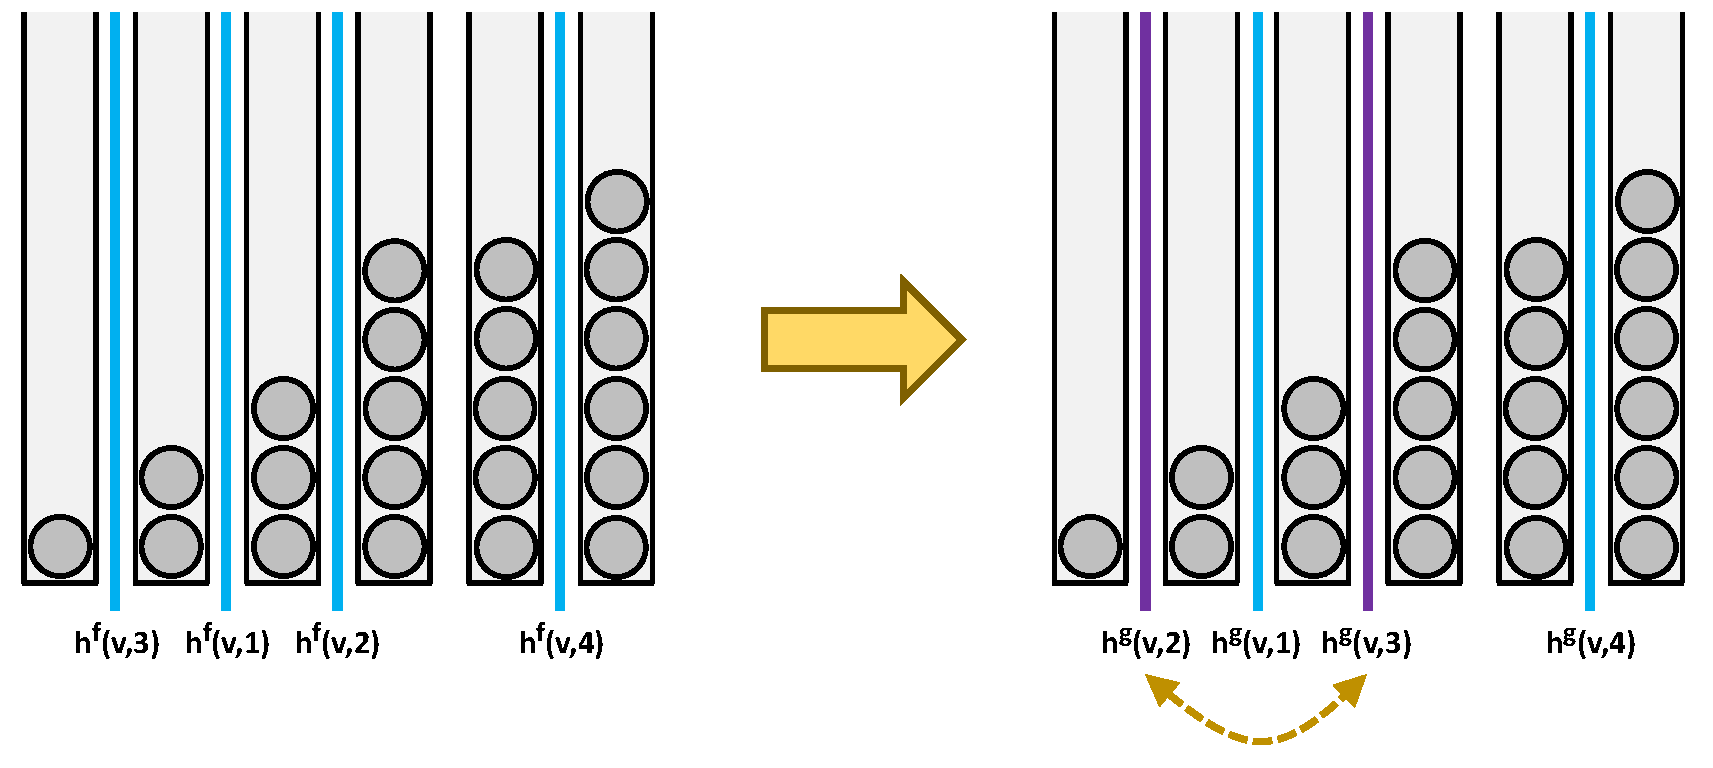
\includegraphics[scale=0.5]{Chapter4/Figs/k_thinning_swap.pdf}
    \caption{The ``swap'' action for \KThinning swapping two subsequent thresholds which were in the wrong order.}
    \label{k-thinning-swap-action}
\end{figure}